
\subsection{Motivación}

\begin{frame}
\frametitle{Motivación}
\begin{itemize}
	\item	Es usual encontrar contextos de aplicación en los
		cuales la ubicación geográfica de los datos a representar
		adquiere una importancia fundamental a la hora de
		recuperarlos. \pause \\

	\item	Tanto es asi que se han desarrollado sistemas de
		bases de datos específicamente orientados a manejar
		eficientemente estos datos. \pause \\

	\item	Algunos ejemplos tangibles de tales contextos son: \pause
	\begin{itemize}
		\item	Servicios web (encontrar el servidor más cercano al cliente) \pause
		\item	Astronomía (encontrar todas las estrellas cercanas a un punto) \pause
		\item	Compañía de seguros (¿qué casas están más expuestas a desastres naturales?) \pause
		\item	Control de aerolíneas (¿dónde está cada avión?)
	\end{itemize}
\end{itemize}
\end{frame}

\begin{frame}
\frametitle{Definición de DB espacial}
\begin{itemize}
	\item	Una base de datos espacial es una DB que provee
		soporte interno para manejar eficientemente datos espaciales. \pause

	\item	Deben proveer ADTs espaciales y extensiones al lenguaje para manejarlos. \pause

	\item	La mayoría permite representar objetos geométricos como puntos,
		lineas y polígonos; pero algunas además se extienden a estructuras
		más complejas como objetos tridimensionales. \pause

	\item	Implementan un indexado espacial, más eficiente que el indexado
		tradicional para estos dominios de aplicación; algoritmos optimizados
		para procesar operaciones espaciales, y reglas para agilizar las consultas.
\end{itemize}
\end{frame}

\begin{frame}
\frametitle{Índices espaciales}
\begin{itemize}
	\item	Aunque existen muchas implementaciones de índices espaciales,
		el método preferido se conoce como {\bf árbol-R}, una estructura
		de datos en forma de árbol de búsqueda balanceado, en donde los
		objetos cercanos se agrupan en su rectángulo delimitador mínimo
		({\it minimum bounding rectangle}), ubicado un nivel más alto que
		ellos (la ``R'' en el nombre del índice es por ``rectángulo'').
		\pause

	\item	En las hojas se encuentran los objetos de nuestra base de datos. \pause

	\item	Este índice hace muy efectiva la búsqueda de los k vecinos más próximos
		a través de un join espacial.
\end{itemize}
\end{frame}

\begin{frame}
\frametitle{Ejemplo de árbol-R}

	\begin{figure}
	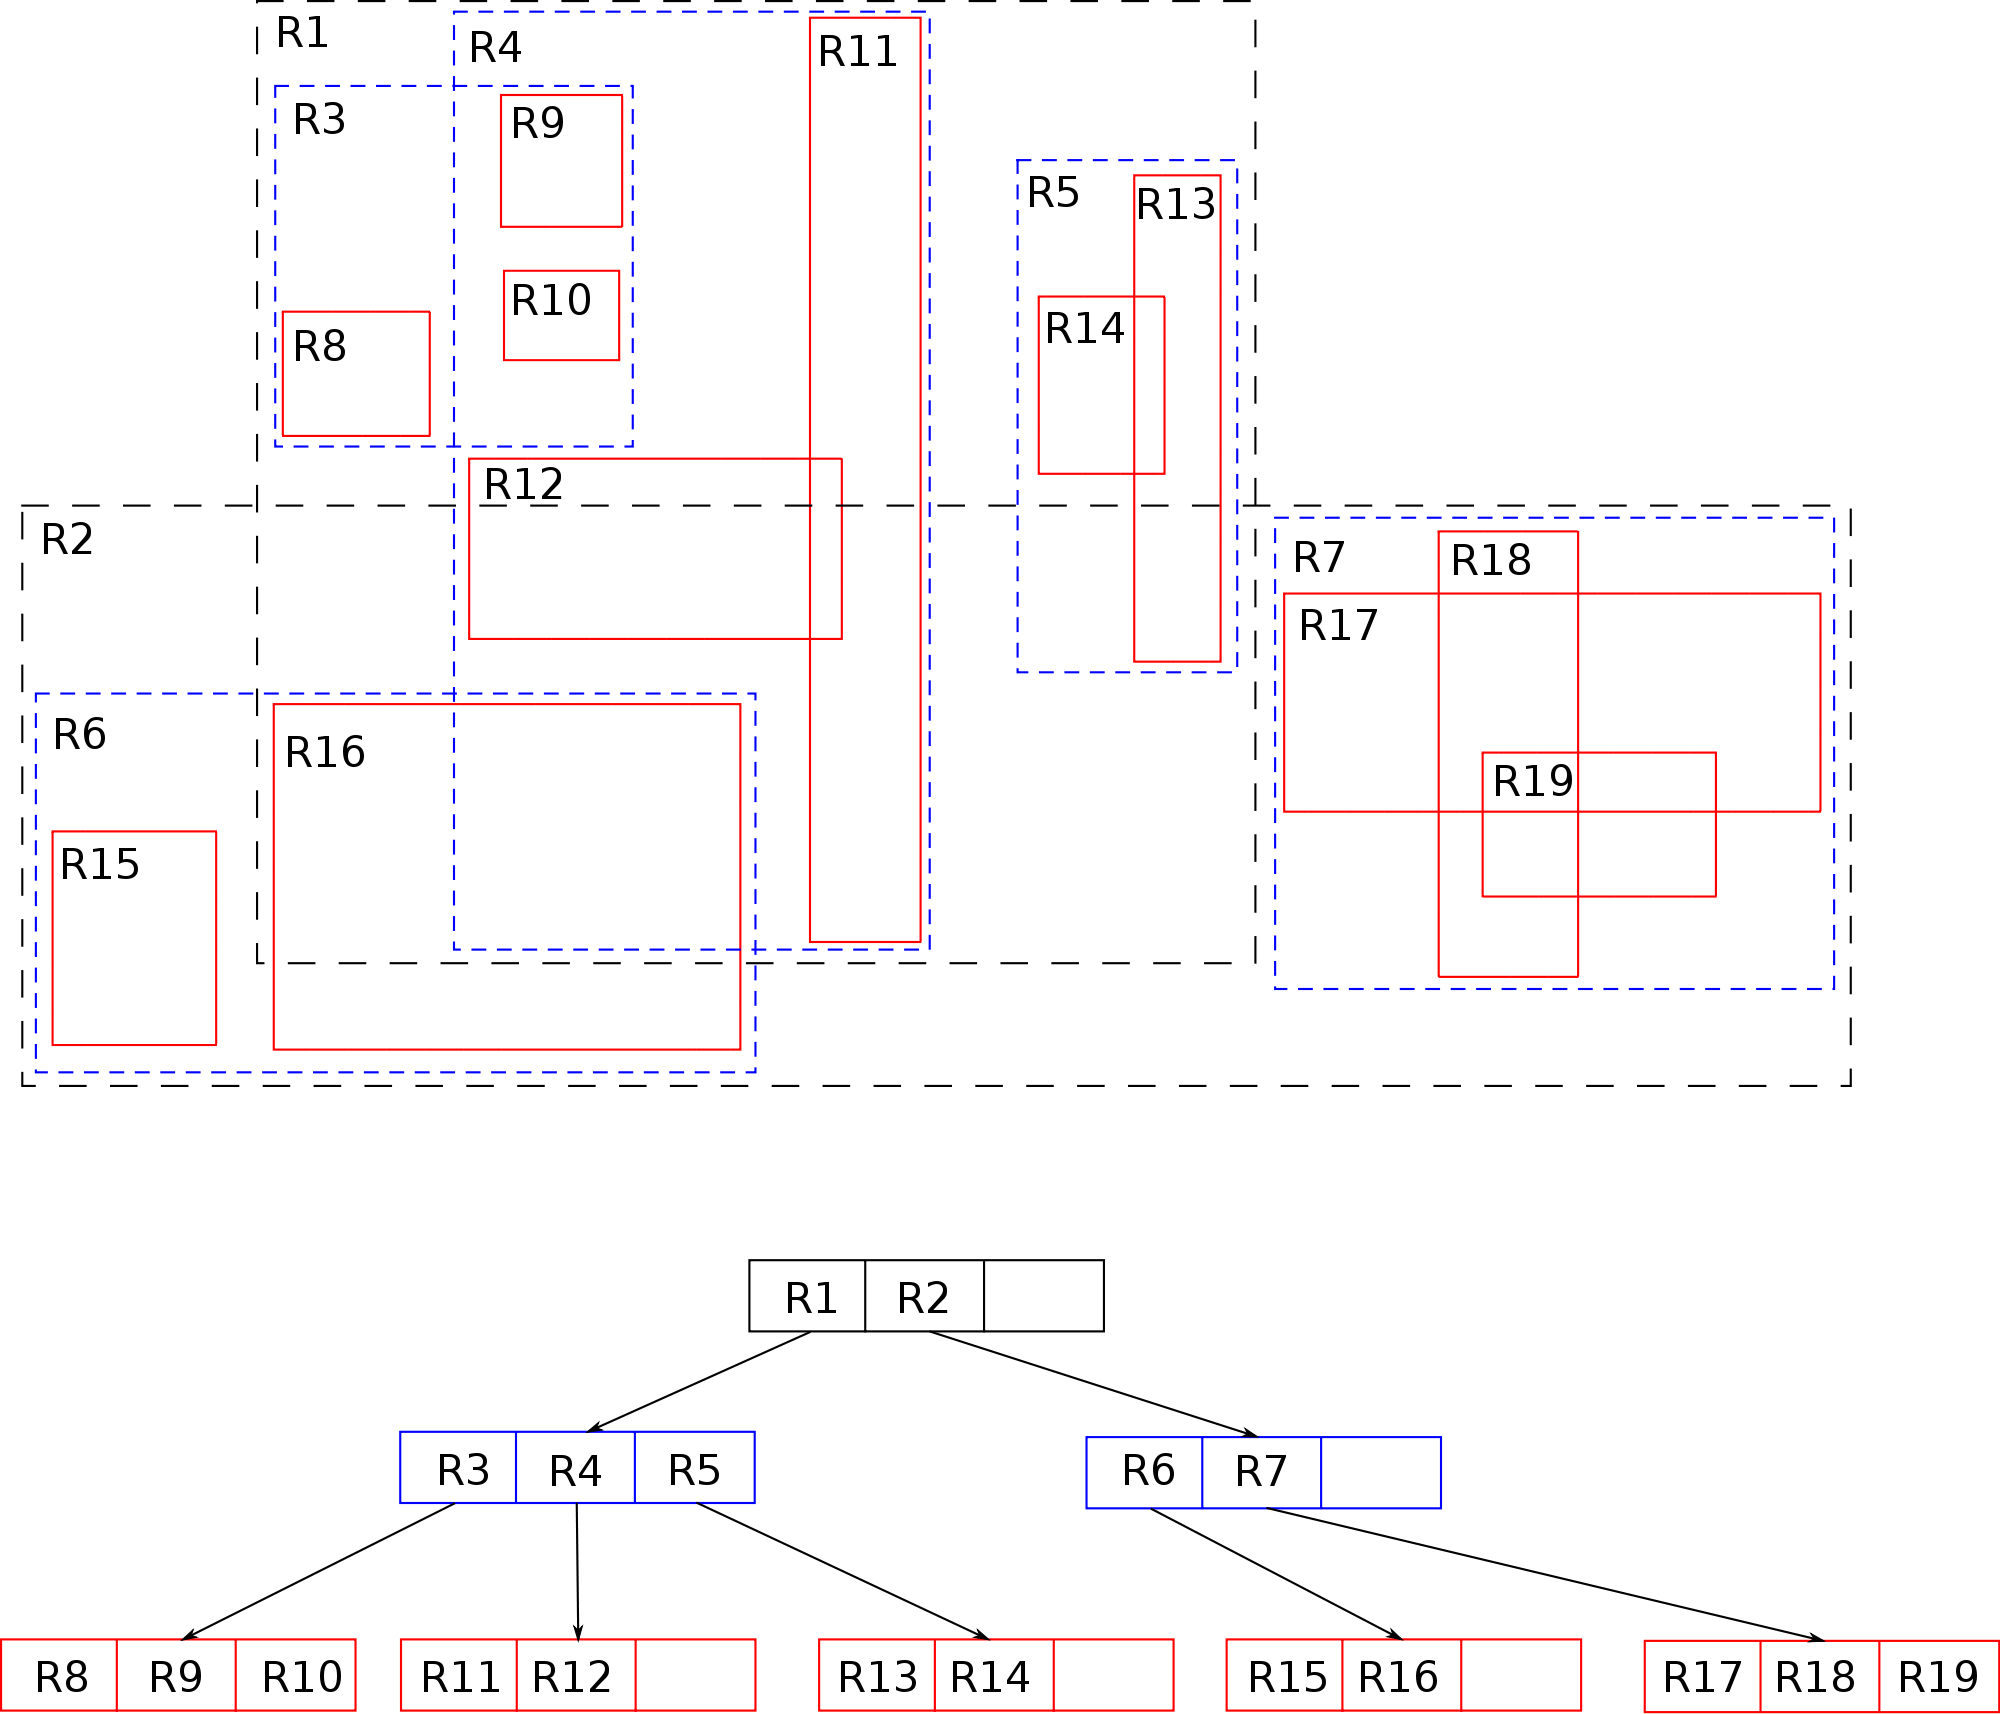
\includegraphics[scale=0.125]{R-tree}
	\end{figure}
\end{frame}

\begin{frame}
\frametitle{Lenguaje de consultas espaciales}
\begin{itemize}
	\item	El comité OGC (Open Geospatial Consortium, alguna vez llamado OGIS),
		conformado por miembros de las mayores compañías de software, formuló
		un estándar sobre la interoperabilidad de intercambio de geodatos. En
		particular, nos interesa la extensión de SQL que se desarrolló al
		respecto. \pause

	\item	La misma se basa en un modelo de datos geométricos, en donde se
		define una clase base no instanciable \texttt{Geometry} y 4 subclases
		principales derivadas de ella, \texttt{Point}, \texttt{Curve},
		\texttt{Surface} y \texttt{GeometryCollection}.
\end{itemize}
\end{frame}

\begin{frame}
\frametitle{Operaciones sobre formas}
\begin{itemize}
	\item	Asociada a cada clase existe un conjunto de operaciones que actúan
		sobre instancias de ellas, las cuales pueden dividirse en tres grandes
		grupos: \pause

		\begin{itemize}
			\item Funciones básicas: aplicables a cualquier instancia de
			\texttt{Geometry}. Por ejemplo, la función para obtener el sistema de
			coordenadas subyacente (\texttt{SpatialReference()}). \pause

			\item Operaciones que predican sobre relaciones entre objetos
			espaciales. Por ejemplo, \texttt{intersect} comprueba si el interior de
			dos objetos no tienen una intersección nula. \pause

			\item Operaciones generales para el análisis espacial. Por ejemplo,
			\texttt{distance} retorna la distancia más corta entre dos objetos
			espaciales.
		\end{itemize}
\end{itemize}
\end{frame}

\begin{frame}
\frametitle{Lenguaje de consultas espaciales}
	La siguiente tabla muestra las operaciones más importantes definidas
	por el estándar OSGI para SQL, discriminadas por el criterio recién
	presentado: \\

	\begin{center}
	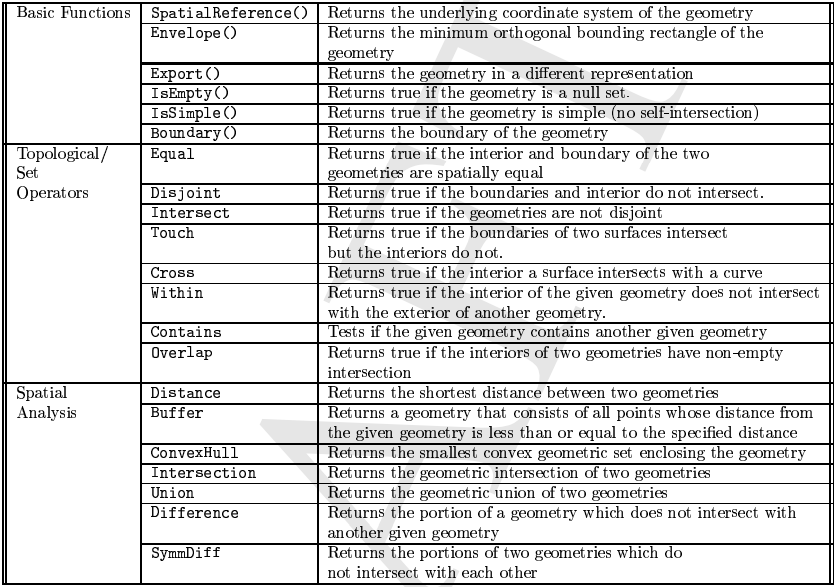
\includegraphics[height=5cm]{tablaOGIS.png}
	\end{center}
\end{frame}

\begin{frame}
\begin{itemize}
	\frametitle{Ejemplos de consultas espaciales}

	\item Consultaremos una base de datos llamada \texttt{Mundo},
	que almacena las relaciones espaciales entre tres entidades:
	\texttt{País}, \texttt{Ciudad} y \texttt{Río}. Las tablas de los tres
	tipos básicos son las siguientes: \pause

	\texttt {
	\item	TABLE Country(Name varchar(30), Cont varchar(30), \\
		~~~~~~~~~~~~~~Pop Integer, GDP Number, \\
		~~~~~~~~~~~~~~Shape Polygon);
	}

	\texttt {
	\item	TABLE City(Name varchar(30), Country varchar(30), \\
		~~~~~~~~~~~Pop Integer, Shape Point);
	}


	\texttt{
	\item	TABLE River(Name varchar(30), Origin varchar(30), \\
		~~~~~~~~~~~~Length Number, Shape LineString);
	}
\end{itemize}
\end{frame}

\begin{frame}
\frametitle{Ejemplos de consultas espaciales: número 1}
\begin{itemize}
	\item	Para obtener los nombres de los países limítrofes con
		Argentina, realizamos la siguiente consulta:
	\pause

	\texttt{
	\item	SELECT~C1.Name AS "Países limítrofes \ \\
		~~~~~~~~~~~~~~~~~~~de Argentina" \\
		FROM~~~Country C1, Country C2 \\
		WHERE~~Touches(C1.Shape, C2.Shape) = 1 \\
		~~~~~~~AND C2.Name = 'Argentina'
	}

	\pause

	\item	El predicado \texttt{Touches} permite conocer si dos objetos
		geométricos son adyacentes sin solaparse.
\end{itemize}
\end{frame}

\begin{frame}
\frametitle{Ejemplos de consultas espaciales: número 2}
\begin{itemize}
	\item	Longitud de la sección de cada río, en cada país que el mismo
		cruza.
	\pause

	\texttt{
	\item	SELECT~~R.Name, C.Name, \\
		~~~~~~~~Length(Intersection(R.Shape, C.Shape)) \\
		FROM~~~~River R, City C \\
		WHERE~~~Cross(R.Shape, C.Shape)
	}
	\pause

	\item	La función \texttt{Intersection} retorna un tipo geométrico (en este
		caso, un \texttt{LineString}). Su longitud será la del río en el
		interior de determinado país.
	\pause

	\item	El predicado \texttt{Cross} indica si el interior de una superficie se
		intersecta con una curva.
\end{itemize}
\end{frame}

\begin{frame}
\frametitle{Ejemplos de consultas espaciales: número 3}
\begin{itemize}
	\item	Ordenar países por cantidad de vecinos.
	\pause

	\texttt{
	\item	SELECT~~~C0.Name, Count(C1.Name),	\\
		FROM~~~~~Country C0, Country C1		\\
		WHERE~~~~Touch(C0.Shape, C1.Shape)	\\
		GROUP~BY~C0.Name			\\
		ORDER~BY~Count(C0.Name)
	}
\end{itemize}
\end{frame}
